\documentclass{beamer}
\usepackage{graphicx}
\usepackage{hyperref}
\usepackage[all]{xy}
\newcommand{\comment}[1]{\textcolor{red}{#1}}
\newcommand{\verify}[1]{\textcolor{blue}{\textbf{#1}}}
\newcommand{\falsify}[1]{\textcolor{red}{\textbf{#1}}}
\usepackage[utf8]{inputenc}
\usepackage[T1]{fontenc}
% Or whatever. Note that the encoding and the font should match. If T1
% does not look nice, try deleting the line with the fontenc.

\setbeamertemplate{frametitle continuation}[from second]

% \mode<presentation>
% {
%   \usetheme{Warsaw}
%   % or ...

%   \setbeamercovered{transparent}
%   % or whatever (possibly just delete it)
% }


\title{Why property-based testing matters}

\author[Pedro Vasconcelos]{Pedro Vasconcelos \\ \texttt{pbvascon@fc.up.pt}}

\institute[LIACC, DCC/FCUP]{
  Laboratório de Inteligência Artificial e Ciência de Computadores\\
  Departamento de Ciência de Computadores \\
  Faculdade de Ciências, Universidade do Porto
}


\newcommand{\bs}{\symbol{92}}

% discard trial for counter-example
\newcommand{\discard}[1]{\textcolor{red}{#1}}
\newcommand{\counter}[1]{\textbf{#1}}
\newcommand{\grayed}[1]{\textcolor{gray}{#1}}

\newcommand{\conc}{\ensuremath{\!+\!\!+}}

% If you have a file called "university-logo-filename.xxx", where xxx
% is a graphic format that can be processed by latex or pdflatex,
% resp., then you can add a logo as follows:

% \pgfdeclareimage[height=0.5cm]{university-logo}{university-logo-filename}
% \logo{\pgfuseimage{university-logo}}



% Delete this, if you do not want the table of contents to pop up atr
% the beginning of each subsection:
%\AtBeginSubsection[]
%{
%  \begin{frame}<beamer>
%    \frametitle{Overview}
%    \tableofcontents[currentsection,currentsubsection]
%  \end{frame}
%}


% If you wish to uncover everything in a step-wise fashion, uncomment
% the following command: 

%\beamerdefaultoverlayspecification{<+->}


\begin{document}

\begin{frame}
  \titlepage
\end{frame}

\begin{frame}
  \frametitle{Overview}
  
  \begin{itemize}
  \item A long-standing challenge for software engineering 
    is ensuring software correctness
  \item Formal proofs are (still) very rarely done
  \item \emph{Tests} are the most commonly used
    techniques
  \item \emph{Types} are the other one (for another talk!)
  \item \emph{Unit tests} are the industry-standard
    for verification ``in the small''
\end{itemize}
\end{frame}

\begin{frame}[fragile]
  \frametitle{Unit tests}
\begin{itemize}
\item Code fragments for testing functions, classes, libraries, etc.
\item Express the expected behaviour for a specific combinations of inputs
\end{itemize}
\medskip

Example: testing an integer square root function in Python.
\begin{verbatim}
def test_isqrt():
   assert isqrt(0) == 0
   assert isqrt(2) == 1
   assert isqrt(4) == 2
   assert isqrt(5) == 2
   assert isqrt(9) == 3
\end{verbatim}

\end{frame}


\begin{frame}[fragile]
  \frametitle{Problems with unit tests}

  Cognitive bias:
  \begin{itemize}
  \item how can we include an edge case in the tests
    that we didn't consider in the code?
  \end{itemize}
  \medskip
  
  Poor scaling:
  \begin{itemize}
  \item a few unit tests per feature
  \item for $n$ features, $O(n)$ unit tests
  \item but testing \emph{interaction} between features require $O(n^2),
    O(n^3), \ldots$ unit tests
  \end{itemize}
  \pause
  \bigskip
  
  Solution:

    \begin{minipage}{0.6\textwidth}
      \begin{quote}
        ``Don't write tests \\
        --- generate them!''
      \end{quote}
      John Hughes, co-author of QuickCheck
    \end{minipage}
    \begin{minipage}{0.3\textwidth}
      \hfill
      
\includegraphics[width=0.8\textwidth]{images/john-hughes}
    \end{minipage}
  
\end{frame}

\begin{frame}[allowframebreaks]
  \frametitle{Property-based testing}

\begin{itemize}
\item Write \emph{properties} instead of specific tests
\begin{itemize}
\item should be universal, i.e.\@ hold for all values
\item should define the expected behaviour for \emph{all} cases
\end{itemize}
\item Specify \emph{generators} for the inputs
\item The testings framework runs the property with
  a large number of inputs
  \begin{itemize}
  \item testing fails if a \alert{counter-example} is found
  \item otherwise, testing succeeds
  \end{itemize}
\end{itemize}

\framebreak

\begin{itemize}
\item QuickCheck (2000): first PBT library (for Haskell)
\item Implementations for other languages
  \begin{description}
    \item[PropEr] for Erlang
  \item[ScalaCheck] for Scala
  \item[Hypothesis] for Python
  \item[FsCheck] for F\#
  \end{description}
\end{itemize}

\ldots many others: \url{https://en.wikipedia.org/wiki/QuickCheck}
\end{frame}

\begin{frame}[fragile]
  \frametitle{Example property}

  Let us use Hypothesis to
  specify a property for the integer square root function.
  \pause
  \bigskip
  
  Let $r = \texttt{isqrt}(n)$; then
  $r$ should be \emph{largest non-negative integer} such that
  $r^2 \leq n$.
  \pause
  \bigskip
  
\begin{semiverbatim}
from hypothesis import \ldots
import hypothesis.strategies as st

@given(st.integers(min_value=0))
def test_isqrt(n):
    r = isqrt(n)
    assert r>=0 and r**2<=n and (r+1)**2>n
  \end{semiverbatim}

  \hfill (Cue demo.)
\end{frame}

\begin{frame}
  \frametitle{Properties in Hypothesis}

  \begin{itemize}
  \item Properties are \emph{functions}
  \item Should fail if the expected condition is not met
  \item Arguments represent \emph{universally quantified}
    variables
  \item Possible values are described
    by the \texttt{@given} decorator
  \item Values are randomly generated using \emph{strategies}
  \item Module \texttt{hypothesis.strategies} provides:
    \begin{itemize}
    \item \emph{predefined strategies} for basic types
    \item methods for \emph{modifying} and \emph{combining} strategies
    \end{itemize}
  \end{itemize}
\end{frame}

\begin{frame}
  \frametitle{Strategies}

  \begin{description}
  \item[integers()] generate integers
  \item[booleans()] generate True/False
  \item[text()] generate Unicode strings
  \item[lists($s$)] lists of elements given by strategy $s$
    % \item[tuples($s1,s2,\ldots$)] lists of elements given by strategies $s1,s2,\ldots$
    \item[\ldots] many others
  \end{description}
  \bigskip
  
  We can also:
  \begin{itemize}
  \item modify strategies using \emph{parameters} (e.g.\@ \texttt{min\_value})
  \item modify strategies by \emph{mapping} and \emph{filtering}
  \item combine them using some \emph{combinator functions}
  % \item sample them using the \texttt{.example()} method    
  \end{itemize} 
\end{frame}

\end{document}



\begin{frame}[fragile]
  \frametitle{Another example}

\begin{block}{}
\begin{semiverbatim}
prop_revapp :: [\alt<2->{\alert{Int}}{a}] -> [\alt<2->{\alert{Int}}{a}] -> Bool
prop_revapp xs ys = reverse (xs++ys) == 
                    reverse ys ++ reverse xs
\end{semiverbatim}
\end{block}

\begin{itemize}
\item The property holds for lists of \alert{any} type\ldots\pause
\item But we need some concrete type for testing (e.g.\@ \alert{Int})
\begin{verbatim}
> quickCheck prop_revapp
+++ OK, passed 100 tests.
\end{verbatim}
\end{itemize}


\end{frame}

\begin{frame}[fragile]
\frametitle{When a property fails}

\begin{block}{}
\begin{semiverbatim}
prop_revapp' :: [Int] -> [Int] -> Bool
prop_revapp' xs ys = reverse (xs++ys) == 
                     reverse xs ++ reverse ys
                     \alert{-{}- wrong !!!!}
\end{semiverbatim}
\end{block}  

\begin{verbatim}
> quickCheck prop_revapp'
*** Failed! (after 5 tests and 3 shrinks):    
[0]
[1]
\end{verbatim}
The counter-example shown is minimal!

\end{frame}

\begin{frame}
  \frametitle{How QuickCheck works}

\begin{itemize}
\item Tests are generated using \alert{type information}
\item QuickCheck provides generators for:
\begin{itemize}
\item basic types (e.g.\@ Int);
\item common structured types (e.g.\@ lists, tuples).
\end{itemize}
\item Generation is parametrized by \alert{size}
  (try smaller values first)
\item The property is used as a test oracle
\item When the test fails, QuickCheck attempts to
  reduce \alert{shrink} the counter-example.
\item Many customizations:
\begin{itemize}
\item number of tests to generate;
\item maximum size;
\item custom generators and shrinking heuristics;
\item gathering statistical data.
\end{itemize}
\end{itemize}
\end{frame}


\begin{frame}[fragile,allowframebreaks]
  \frametitle{Shrinking}

\begin{block}{}
\begin{semiverbatim}
prop_revapp' :: [Int] -> [Int] -> Bool
prop_revapp' xs ys = reverse (xs++ys) == 
                     reverse xs ++ reverse ys
                     \alert{-{}- wrong !!!!}
\end{semiverbatim}
\end{block}  
\smallskip

Assume we randomly generate
\begin{semiverbatim}
xs = [2,2]
ys = [1]
\end{semiverbatim}
This is a \alert{counter-example} because:
\begin{semiverbatim}
      reverse ([2,2]++[1]) \ensuremath{\neq} 
               reverse [2,2] ++ reverse [1]
\end{semiverbatim}

\pagebreak

%\[ \text{reverse}~([2,2]\conc[1]) \neq \text{reverse}~[2,2] \conc 
%\text{reverse}~[1] \]

Shrinking our counter-example:
\[ \xymatrix@-0.5pc{
  & & \counter{[2,2],[1]}\ar[dll]\ar[dl]\ar[d]\ar[dr]\ar[drr]\ar@{--}[drrr] \\
  \counter{[2],[1]}\ar[d]\ar[dr]\ar[drr]\ar[drrr]\ar[drrrr] & 
  \grayed{[2],[1]} & \grayed{[0,2],[1]} & \grayed{[1,2],[1]} & 
  \grayed{[2,0],[1]} & \grayed{\cdots} \\
  \discard{[\,],[1]} & \counter{[0],[1]}\ar[dl]\ar[d]\ar[dr] &
  \grayed{[1],[1]} & \grayed{[2],[\,]} & \grayed{[2],[0]} \\
  \discard{[\,],[1]} & \discard{[0],[\,]} & \discard{[0],[0]}
} 
\]
\medskip

\begin{itemize}
\item A local miminum is obtained after two steps
\item The shrinking heuristic is \alert{deterministic}  (pure function)
\end{itemize}
\end{frame}



\begin{frame}[fragile]
\frametitle{A larger example}
\framesubtitle{Based on Erlang code from Ericsson}

SMS text packing:
\begin{itemize}
\item 7-bit characters;
\item transmitted using 8-bit \emph{bytes};
\item we can pack eight 7-bit caracteres into 7~bytes
\item two functions:
\begin{verbatim}
pack :: [Byte] -> [Byte]
unpack :: [Byte] -> [Byte]
\end{verbatim} 
\end{itemize}

\begin{block}{Left-inverse property}
\begin{verbatim}
prop_pack txt  = unpack (pack txt) == txt
\end{verbatim}
\end{block}
\end{frame}



\begin{frame}
  \frametitle{Imperative programs}

Can use QuickCheck to test programs that:
\begin{enumerate}
\item modify state;
\item read and write files;
\item use network services, databases, etc.;
\item written in other languages?
\end{enumerate}
\end{frame}

\begin{frame}
\frametitle{Testing imperative programs}

\begin{itemize}
\item Generate sequences of commands
\item Specify behaviour using a functional model
\item Compare execution against the model
\end{itemize}

\begin{center}
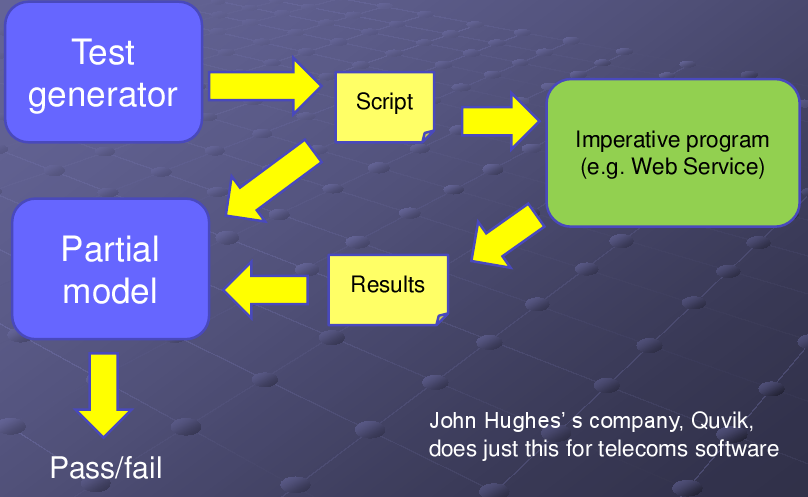
\includegraphics[width=0.75\textwidth]{imperative.png}
\end{center}
\end{frame}


\begin{frame}
\frametitle{Example}


A subset of the C language file API:
\begin{description}
\item [fwrite(buffer, count, stream)] write \emph{count} bytes 
  from \emph{buffer} to \emph{stream}
\item [fread(buffer, count, stream)] read \emph{count} bytes 
  from \emph{stream} to \emph{buffer}
\item [fseek(stream, offset)] set the file position for \emph{stream}
\end{description}
\end{frame}

\begin{frame}[fragile]
\frametitle{Modeling a file}

\begin{itemize}
\item A \emph{list of bytes} and an \emph{index} (position)
\item Functional model specified using standard list functions
\end{itemize}

\begin{center}
\includegraphics[width=0.7\textwidth]{split1} \\
\begin{minipage}{0.7\textwidth}
\begin{verbatim}
(prefix,suffix) = splitAt pos bytes
\end{verbatim}
\end{minipage}
\end{center}


\end{frame}


\begin{frame}[fragile]
  \frametitle{Modeling reading}


\begin{center}
\includegraphics[width=0.7\textwidth]{read1}
\end{center}

\begin{verbatim}
extract :: [Byte] -> Int -> Int -> [Byte]
extract bytes pos count
    = let (_,suffix) = splitAt pos bytes
          (out,_) = splitAt count suffix
      in out
\end{verbatim}


\end{frame}

\begin{frame}[fragile]
  \frametitle{Modeling writing}


\begin{itemize}
\item Similiar to the reading case
\item Exception: extend with zeros when writing after EOF
  (POSIX spec)
\end{itemize}
\begin{center}
\includegraphics[width=0.7\textwidth]{write1}
\end{center}

\begin{semiverbatim}
overwrite :: [Byte] -> Int -> [Byte] -> [Byte]
overwrite bytes pos new
    = let (pre, suf) = splitAt pos bytes
          (_, suf') = splitAt (length new) suf
      in \textbf{extend pre pos 0} ++ new ++ suf'
\end{semiverbatim}
\end{frame}

\begin{frame}[fragile]
\frametitle{Generating commands}

\begin{semiverbatim}
\comment{-{}- abstract syntax for commands}
data Cmd = FWrite [Byte]
         | FRead Int
         | FSeek Int

\comment{-{}- generator for commands}
\comment{-{}- choose read, write, seek with equal probability}
instance Arbitrary Cmd where
    arbitrary = oneof [liftM FWrite arbitrary,
                       liftM FRead filepos,
                       liftM FSeek filepos]

filepos :: Gen Int
filepos = sized (\bs{}n -> choose (0, min n 1000))
\end{semiverbatim}
%NB: o \emph{QuickCheck} gera \emph{sequências}
%usando o gerador dos elementos.
\end{frame}

\begin{frame}[fragile]
\frametitle{Functional model for a command}

\begin{itemize} 
\item File model is a \alert{pair}: list of bytes, position
\begin{verbatim}
type FileModel = ([Byte], Int) 
\end{verbatim}
\item First approximation: commands are \alert{transition functions}
\item But they also yield a \alert{result}:
\begin{description}
\item [\texttt{fread}:] the list of \emph{bytes} read;
\item [\texttt{fwrite}, \texttt{fseek}:]  nothing  (``void'' result)
\end{description}
\end{itemize}
\end{frame}


\begin{frame}[fragile]
  \frametitle{Modeling a command sequence}

\begin{itemize}
\item Initial state is an empty file
\item Run state transitions
\item Acumulate any read results 
\end{itemize}

\begin{description}
\item[Example] \verb|[FWrite [2,3,7], FSeek 1, FRead 2]|
\item[Results] \verb|[Nothing, Nothing, Just [3,7]]|
\end{description}

\begin{center}
\includegraphics[width=\textwidth]{state2}
\end{center}


\end{frame}


\begin{frame}[fragile]
  \frametitle{C code generation}


\begin{center}
 \texttt{[FWrite [2,3,7], FSeek 1, FRead 2]}  
\end{center}
\begin{block}{}
{\tiny
\begin{columns}[t]
\begin{column}{0.4\textwidth}
\begin{verbatim}
/* This file is an automatically 
   generated test script */
#include <stdio.h>
#define NL              printf("\n")
#define OPEN            printf("[")
#define CLOSE           printf("]")
#define COMMA           printf(",")
#define JUST            printf("Just ")
#define NOTHING         printf("Nothing")

/* global read buffer */
static unsigned char buffer[10000]; 

/* output n bytes in Haskell syntax */
void LIST(int n) { 
  int i;
  OPEN;
  if (n>0) printf("%d", (int)buffer[0]);
  for(i=1; i<n; i++) 
    printf(", %d",(int)buffer[i]);
  CLOSE;
}
\end{verbatim}
\end{column}
\begin{column}{0.5\textwidth}
\begin{verbatim}
static unsigned char data0[] = {2,3,7};

int main() {
FILE *stream = tmpfile();
OPEN;
NOTHING; fwrite(data0,1,3,stream);
COMMA;
NOTHING; fseek(stream,1,SEEK_SET);
COMMA;
JUST; LIST(fread(buffer,1,2,stream));
CLOSE;
NL;
fclose(stream);
return 0;
}
\end{verbatim}
\end{column}
\end{columns}}
\end{block}
\end{frame}



\begin{frame}[fragile]
  \frametitle{Correcteness property}

For \alert{all command sequences},  evaluating the 
functional model and the compiled C code yield the same results.
\begin{verbatim}
prop_filemodel :: [Cmd] -> Property
prop_filemodel cmds 
    = monadicIO $
      do out <- run (testScript cmds)
         assert (out == testModel cmds)
\end{verbatim}
\end{frame}

\begin{frame}[fragile]
  \frametitle{Checking this property}

\begin{verbatim}
> quickCheck prop_filemodel 
*** Failed! (after 159 tests and 16 shrinks):    
[FSeek 1,FWrite [],FSeek 0,FRead 1]
\end{verbatim}

What went wrong?\pause
\medskip


Our functional model is incorrect: writing zero bytes should \emph{not} 
extend the file!
\end{frame}


\begin{frame}[fragile]
\frametitle{Checking again (after correcting)}

\begin{verbatim}
> quickCheck prop_filemodel
+++ OK, passed 100 tests.
\end{verbatim}

\begin{itemize}
\item Passed 100 random tests cases
\item We could pursue this further:
\begin{itemize}
\item increase the number of tests;
\item increase the test case size;
\item gather statistics.
\end{itemize}
\end{itemize}
\end{frame}

\begin{frame}
\frametitle{Partial specifications}


\begin{itemize}
\item It is not always possible to write a full functional model
\begin{itemize}
\item can be too complex;
\item doubles the development effort (model and implementation).
\end{itemize}
\item Alternative: write properties based on partial
  specifications
\end{itemize}
\end{frame}

\begin{frame}
  \frametitle{Observational equivalence}


$$ \texttt{[FWrite~[1,2],~FWrite~[3]]} \simeq
\texttt{[FWrite~[1,2,3]]} $$
\bigskip
\pause

\begin{block}{$cmds_1 \simeq cmds_2$}
For all contexts $C[\cdot]$,
the \alert{observable results} of executing $C[cmds_1]$ e $C[cmds_2]$
are equal.
\end{block}

\end{frame}


\begin{frame}[fragile]
  \frametitle{Observational equivalence in QuickCheck}


\begin{verbatim}
(==~) :: [Cmd] -> [Cmd] -> Property
cmds1 ==~ cmds2 
      = forAll arbitrary $ \pre ->
        forAll arbitrary $ \suf ->
        monadicIO $
        do out1<-run (obsScript (pre++cmds1++suf))
           out2<-run (obsScript (pre++cmds2++suf))
           assert (out1 == out2)
\end{verbatim}


\begin{itemize}
\item The \alert{context} is a \emph{prefix} and \emph{sufix} of commands
\item The \alert{observable result} is the sequence of bytes read
\end{itemize}


\end{frame}


\begin{frame}[fragile]
  \frametitle{Testing equivalences}

We can use the observational equivalence relation for testing:
\begin{verbatim}
> quickCheck ([FWrite [1,2],FWrite [3]] ==~ 
              [FWrite [1,2,3]])
+++ OK, passed 100 tests.

> quickCheck ([FWrite [1,2,3]]==~[FWrite [3,2,1]])
*** Failed! (after 4 tests and 3 shrinks):    
[]
[FSeek 0,FRead 1]
\end{verbatim}
The counterexample is a context that distinguishes
the left and right-hand sides.
\end{frame}

\begin{frame}[fragile]
  \frametitle{Some example properties}

\begin{semiverbatim}
\comment{-{}- sucessive writes}
prop_obsWriteSeq xs ys
    = [FWrite xs,FWrite ys] ==~ [FWrite (xs++ys)]

\comment{-{}- sucessive seeks}
prop_obsSeek 
    = forAll filepos $ \bs{}n ->
      forAll filepos $ \bs{}m -> 
      [FSeek n,FSeek m] ==~ [FSeek m]
\end{semiverbatim}
\end{frame}


\begin{frame}
  \frametitle{Industrial use example}

\begin{itemize}
\item Ericsson Media proxy
\item Establish telephony connection throught a firewall
\item Tested with Erlang QuickCheck (Quviq.com)
\item Adding and removing paricipants in a call
\item Random counterexample with 160 commands
\item Shrunk automatically to 7 commands
\end{itemize}

\begin{center}
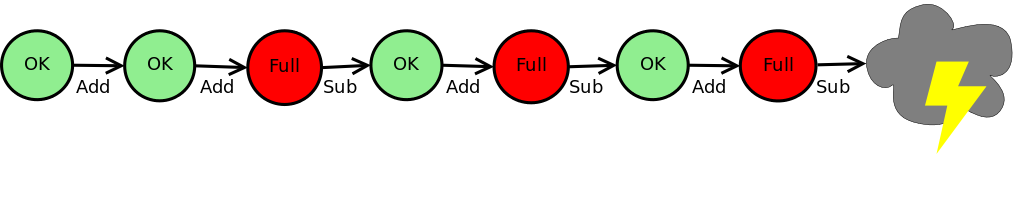
\includegraphics[width=\textwidth]{media1}
\end{center}
\end{frame}



\begin{frame}
  \frametitle{Conclusion}

\begin{itemize}
\item QuickCheck is an \alert{domain-specific language}
  for writing \alert{properties} and \alert{generators}
  embedded in Haskell.
\item Gives a short-term pay-off for writting specifications
\item Flexible: specifications can be based on
  models, observations,  pre-and post-conditions, etc.
\item Widely used in Haskell code
\item Has been ported to many other languages
\end{itemize}
\end{frame}



\begin{frame}
  \frametitle{References}

  \begin{thebibliography}{9}
  \bibitem{QuickCheck00} Koen Claessen \& John Hughes: \newblock
    \emph{QuickCheck: A lightweight tool for random testing
      of Haskell programs}, ICFP 2000.
\bibitem{QuickCheck02} Koen Claessen \& John Hughes: \newblock
  \emph{Testing monadic code with QuickCheck}, 
  Haskell Workshop 2002.
\bibitem{telecoms} Thomas Arts, John Hughes \& Joakim Johansson: \newblock
\emph{Testing Telecoms Software with Quviq QuickCheck}, Erlang'06.
%\bibitem{Fop} Jeremy Gibbons \& Oege de Moor (editors): \newblock
%  \emph{The Fun of Programming}, Palgrave, Macmillan, 2003.
%  http://web.comlab.ox.ac.uk/oucl/publications/books/fop/
\end{thebibliography}
\end{frame}



\end{document}

